\documentclass{article}
\usepackage{graphicx} % Required for inserting images
\usepackage{blindtext}
\usepackage{hyperref}

\title{06-10-2024}
\author{Samuel Fournier (20218212)}
\date{October 2024}

\begin{document}

\maketitle

Dans les deux dernières semaines j'ai travailler sur l'implémentation de la grille de voxels et sur la première version
de l'algorithme de parcours de grille: le DDA-3D. L'implémentation de la grille à causé quelques problèmes. Malgré tout,
son implémentation était assez rapide, car j'avais déjà un template à suivre (les implémentations d'objet fait par
Caio dans le cadre du projet du cours IFT3355). Ensuite, j'ai du implémenter les tests d'intersection entre les
rayons et la grille. Cela a été un peu plus ardu, mais tout de même assez simple. L'idée derrière l'implémentation
était plus ou moins la mème que pour les autres objets du RayTracer que moi et mon coéquipier avions fait lors de la
session d'hiver 2024. L'endroit où j'ai vraiment bloqué, était l'implémentation du DDA-3D. J'ai lu plusieurs articles
ainsi que des messages sur des forums comme StackOverflow et je comprenais l'idée générale de l'algorithme, mais
certaines des formules mathématiques (le calcule du tDeltaXYZ entre autres) ne faisait aucun sens où était très mal
expliqué. Cependant, j'ai réussi à implémenter l'algorithme malgré tout. J'ai emprunter les concepts que je
comprennait des articles et messages et implémenter moi même les parties plus flou. Il est possible que ma version
soit peu performante à cause de ça, mais c'est le moindre de mes soucis en ce moment. En plus d'avoir un algorithme
de parcours de grille, j'ai déjà implémenté l'accumulation de densité dans le rayon pour générer un à peu près de nuage.
Par contre, comme je n'ai pas trouvé de ressource en ligne au sujet des formules (pour que ça soit le plus beau et
réaliste possible), je ne fais qu'interpoler mes densités. Je vais continuer de faire mes recherches et j'ai demandé à
Pierre Poulin s'il connaissait les formules ou des ressources qui pourrait m'aider. Généralement, je suis légèrement
en avance sur mon plan. En effet, pour les deux dernières semaines mes deux objectifs principaux étaient d'implémenter
la grille de voxel et d'implémenter le DDA-3D. Cependant, j'ai été en mesure d'implémenter l'accumulation d'opacité et
d'avoir des rendus d'image avec une grille de voxel qui représente un nuage. Mon objectif pour les semaines à venir sont
les suivants:
\begin{itemize}
    \item Implémenter une interpolation TriLinéaire pour calculer les densités pour avoir des densités variés dans un
    voxel, plutôt qu'avoir une densité uniforme.
    \item Paufiner les formules d'accumulation d'opacité et de "coloriage" de voxel.
    \item Implémenter le second algorithme de parcours de grille de voxel: le Ray Marching.
\end{itemize}
Voici quelques rendus que j'ai pus obtenir grâce à mon progrès (pour toute ces scènes, j'ai utiliser
la scène all\_at\_once.ray):
\begin{center}
    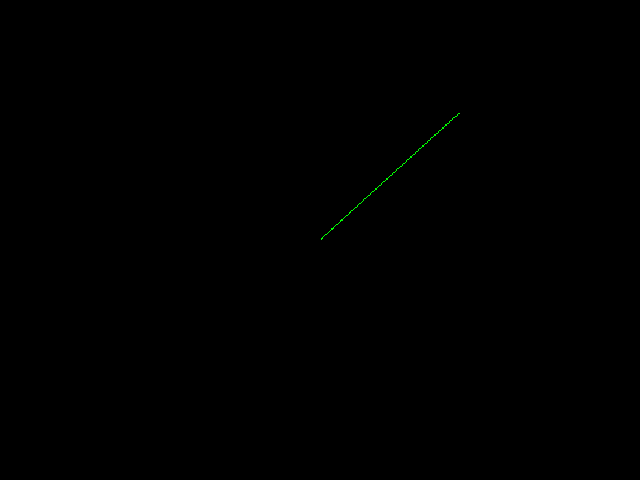
\includegraphics[scale = 0.5]{Images/GrilleDiagonale.png} \\
    Image d'une grille de voxel de 100x100x100 voxels. Preuve que le DDA marchait bel et bien. Si le rayon frappait
    un voxel avec un densité de 0 il l'ignore et si c'est une densité de 1 il le colorie vert.
\end{center}
\begin{center}
    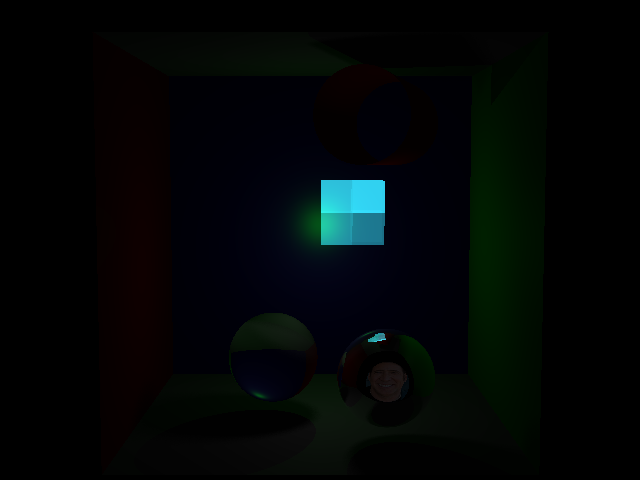
\includegraphics[scale = 0.5]{Images/PremierTest.png} \\
    Premier test de l'accumulation d'opacité sur une grille de 2x2x2 voxels. La couleur des voxels étaient
    mis aléatoirement, mais le restant de la scène devient très sombre par conséquent.
\end{center}
\begin{center}
    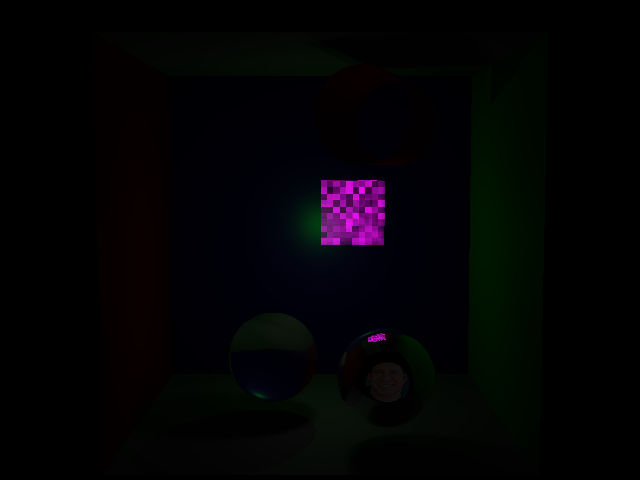
\includegraphics[scale = 0.5]{Images/SecondTest.png} \\
    Même chose que le premier test, mais pour une grille 15x15x15 voxels violets.
\end{center}
\begin{center}
    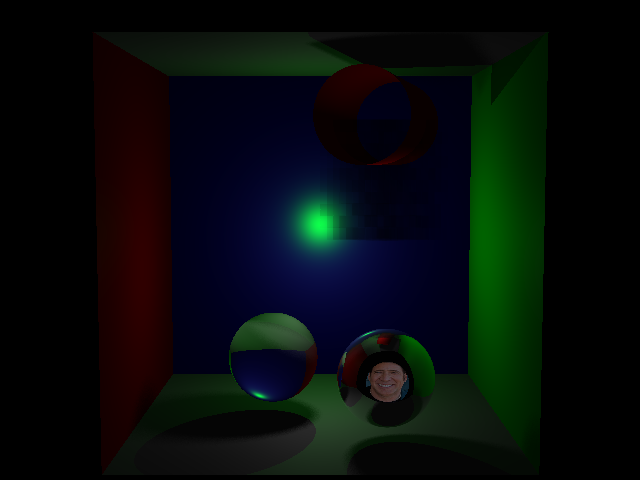
\includegraphics[scale = 0.5]{Images/TroisiemeTest.png} \\
    Ici c'est une grille de 15x15x15 voxels, mais cette fois si avec aucune couleur. Par conséquent,
    l'image est moins sombre et les voxels prennent un peu la couleur de ce qui est derrière eux.
\end{center}
Voici le lien au Paper que j'ai utiliser pour comprendre l'algorithme de DDA:
\href{http://www.cse.yorku.ca/~amana/research/grid.pdf}{A Fast Voxel Traversa;
Algorithm for Ray Tracing (John Amanatides \& Andrew Woo} et voici le lien à un repo Github qui a implémenter
l'algorithme en C++ et explique plus en détail certains des concepts:
\href{https://github.com/cgyurgyik/fast-voxel-traversal-algorithm/blob/master/overview/FastVoxelTraversalOverview.md}
{Gyurgyik C \& Kellison A}

\end{document}
